In this section we explore the effect of varying the underlying binary physics assumptions, both on the detection rate (Section~\ref{sec:detection_rate_analysis}) and the properties of the detectable systems (Section~\ref{sec:property_variations}).

\subsection{Detection rates}\label{sec:detection_rate_analysis}
In Figure~\ref{fig:detection_rates}, we show the expected number of LISA detections for each model variation and discuss the prominent trends in the following sections. For the exact rates and uncertainties plotted in this figure see Table~\ref{tab:detection_rates}.

The BHBH detection rate is markedly robust across variations of physics assumptions, as can be seen in the top panel of Figure~\ref{fig:detection_rates}, with the mean detections in three quarters of our models staying within 25\% of the fiducial rate. In contrast, the BHNS detection rate is very sensitive to all changes that we made in our binary physics assumptions, varying across two orders of magnitude in the middle panel of Figure~\ref{fig:detection_rates}. Finally, in the last panel of Figure~\ref{fig:detection_rates} we show that the NSNS detection is only moderately sensitive to certain changes in physics assumptions, varying by up to an order of magnitude, whilst showing no change for many models.

\begin{figure*}[p]
    \centering
    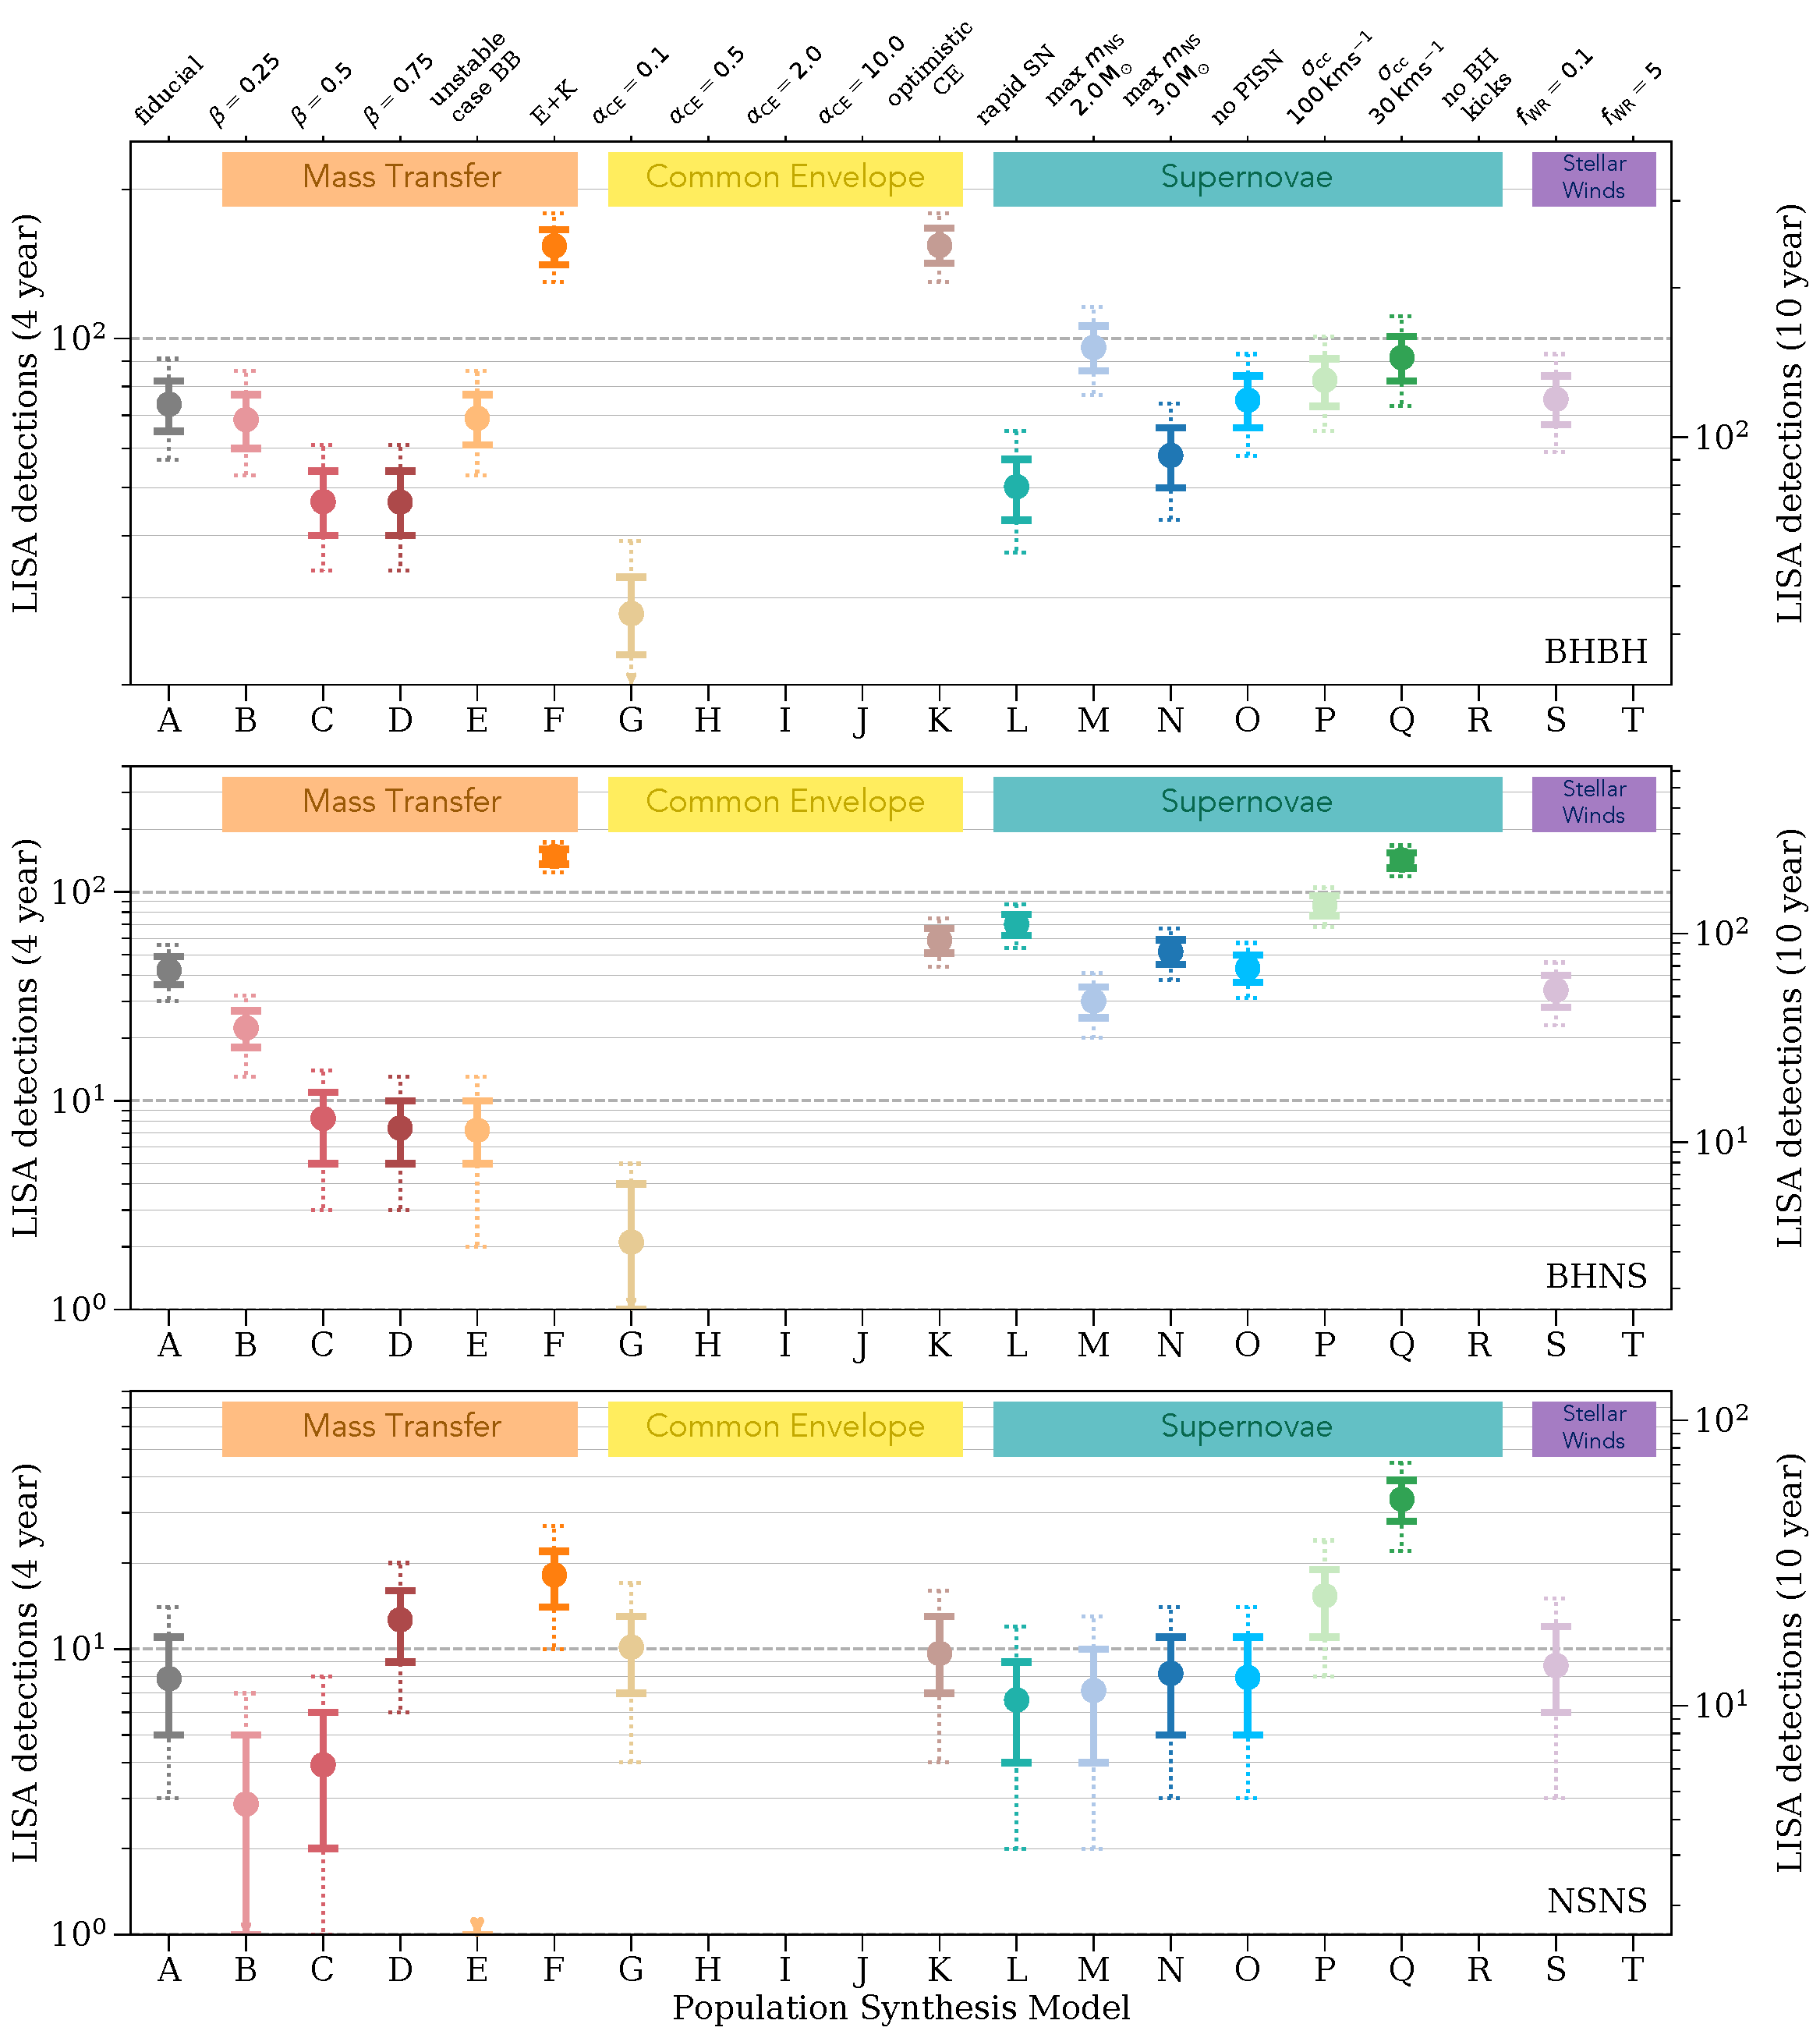
\includegraphics[width=\textwidth]{3_dco_detections.pdf}
    \caption{The number of expected detections in the LISA mission for different DCO types and model variations. Error bars show the 1- (solid) and 2-$\sigma$ (dotted) Poisson uncertainties. An arrow indicates that the error bar extends to zero. The left axis and grid lines show the number of detections in a 4-year LISA mission and the right axis shows an approximation of the number of detections in a 10-year mission (we scale the axis by $\sqrt{T_{\rm obs}}$, see Table~\ref{tab:detection_rates} for exact rates). Each model is described in further detail in Table~\ref{tab:physics_variations} and details of the fiducial assumptions are in Section~\ref{app:fiducial_physics}. See Sec.~\ref{sec:detection_rate_analysis} for a discussion. \todo{Will add H, I, J, R, T once Floor says that they are done}}
    \label{fig:detection_rates}
\end{figure*}

\subsubsection{Mass transfer variation trends}

In models \modBetaLow{}-\modBetaHigh{}, we set the mass transfer efficiency $\beta$ to a fixed value. For the BHBHs and BHNSs, as we increase $\beta$ the detection rates steadily decrease. This may seem unintuitive since one may assume that a higher mass transfer efficiency would lead to more massive compact objects and thus a more detectable population. However, this contributes to the envelope mass and so without increasing the core mass or fallback rate, the final compact object mass is relatively unaffected. Moreover, one must consider that most of these DCOs are formed through a common envelope event and so retaining more of the envelope during mass transfer means that the eventual ejection of the envelope is much more difficult, thus leading to more stellar mergers and fewer detectable systems \citep[e.g.][]{Kruckow+2018}.

In contrast, for the NSNSs, the detection rate increases with increasing $\beta$. This is for two main reasons: firstly the ejection of a common envelope is less problematic for NSNSs as they are less massive \citep[e.g.][]{Kruckow+2018}. Moreover, the increased mass transfer efficiency means that systems that were previously below the mass necessary to become a NS can now accrete enough mass to form a NS. Although the same is true for more massive stars becoming BHs instead of NSs, due to the IMF, there is a net flux of more stars becoming NSs.

Enforcing that case BB mass transfer is always unstable (model \modCaseBB{}) has little effect on the BHBH detection rate whilst moderately and drastically decreasing the detection rates of BHNSs and NSNSs respectively. This is because a large fraction of NSs (and the majority of NSNS binaries are formed) through case BB mass transfer. Therefore, setting this mass transfer to be always unstable results in many of these binaries to merge before they could become DCOs since we assume the pessimistic common envelope (CE) scenario by default.

If we instead use the optimistic CE scenario when setting case BB mass transfer to be unstable (model \modCaseBBOpt{}) we find that the rates instead uniformly increase across DCO types. This is both from the natural increases from using the optimistic CE scenario (see Sec.~\ref{sec:detection_rate_CE_trends} in which we discuss model \modOpt{}), as well as additional increases from adding more DCOs formed through CE events after case BB mass transfer. This explains why we see more detections for BHNSs and NSNSs in model \modCaseBBOpt{} than in model \modOpt{}.

\subsubsection{Common envelope variation trends}\label{sec:detection_rate_CE_trends}

\todo{Discuss $\alpha_{\rm CE}$ changes once Floor ready}

We explore the optimistic CE scenario in model \modOpt{}, meaning that we allow Hertzsprung gap donors to survive CE events. A large fraction of the progenitors of the BHs in our sample expand significantly during the Hertzsprung gap phase and initiate CE events. Therefore, though the detectable \textit{fraction} does not change significantly, the increased formation rate of BHs in the Milky Way leads to this model predicting significantly more BHBH detections. This increase is less significant for BHNSs since their progenitors tend to be less massive and thus initiate CE events during the Hertzsprung gap less frequently. For the same reason, the NSNS detection rate shows little significant change.

\subsubsection{Supernova variation trends}

Changes to the remnant mass prescription (models \modRapid{}-\modNSHigh{}) have no effect on the NSNS detection rate for two reasons. A large fraction of the NSs in our sample are formed through ECSN, in which case their masses are set to $1.26 \unit{M_\odot}$ regardless of the remnant mass prescription. Secondly, the majority of the remaining NSs have such low progenitor masses that they are set to the lowest remnant mass in the prescription ($1.28 \unit{M_\odot}$ for the delayed prescription and $1.1 \unit{M_\odot}$). This means that changing the upper portion of the mass range of NSs in the remnant mass prescription has little effect.

This is not the case for BHBHs and BHNSs. The different remnant mass prescriptions and maximum neutron star masses change whether a progenitor becomes a black hole or a neutron star. Hence, using the rapid prescription (model \modRapid{}) or increasing the maximum neutron star mass (model \modNSHigh{}), means that more progenitors form high mass NSs rather than low mass BHs and so more BHNSs are formed. This explains the higher detection rates for BHNSs and lower detection rates for BHBHs in these models. The inverse is true for model \modNSLow{}, where instead more BHBHs are formed and detected.

Additionally, we find that not implementing PISN and PPISN (model \modNoPISN{}) has no effect on the results for any DCO type. This is because the average metallicity of the Milky Way is high enough than no progenitor retains enough mass to initiate a PISN or PPISN.

Decreasing the core-collapse supernova velocity dispersion (models \modSigLow{}-\modSigLower{}) increases the detection rates for each DCO type since lower kicks result in fewer disrupted binaries and hence a more numerous detectable population. This increase is least prominent for BHBHs since their increased mass mean that disruptions are less frequent than, for instance, in NSNSs. It is also notable that \citet{Broekgaarden+2021} found that these two models best matched the detection rates from LIGO. Therefore we find the best matching models for the LIGO detection rates also produce the highest LISA detection rates.

\todo{dicuss no BH kick when done}
%The model with no BH kick (\modNoBH{}) is slightly lower than model \modSigLower{} as the number of surviving binaries is limited by the neutron star kick more than the black hole kick.

\subsubsection{Stellar wind variation trends}
\todo{}

\subsection{Properties of detectable systems}\label{sec:property_variations}
\todo{Describe the plots -- also explore whether there is anything interesting the CE ones once they are done}

\begin{figure}[htb]
    \centering
    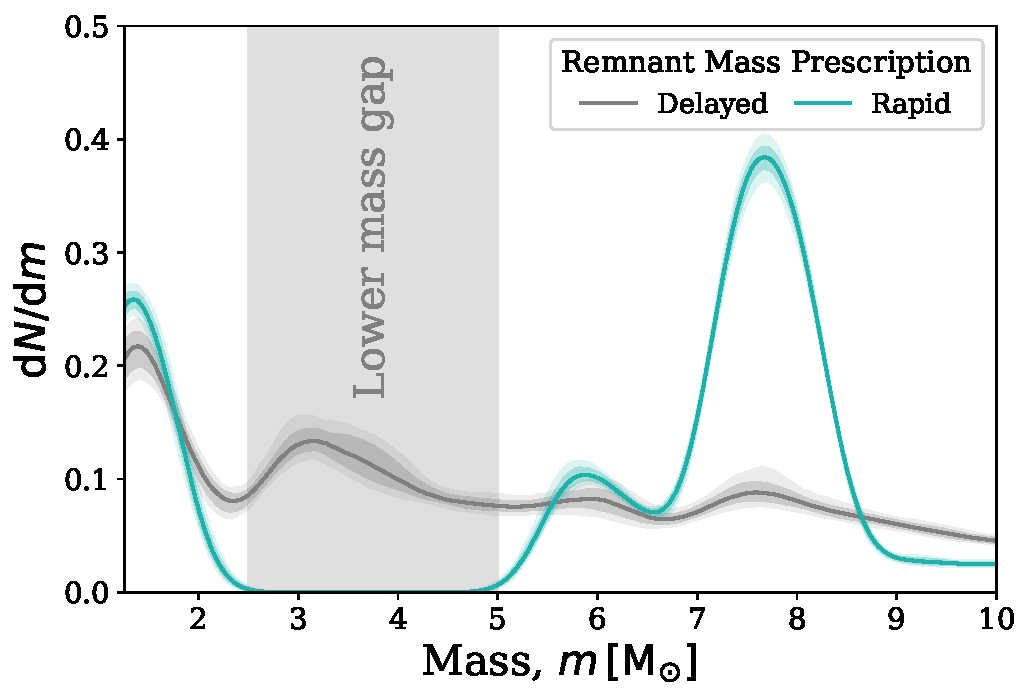
\includegraphics[width=\columnwidth]{lower_mass_gap_rapid_variation.pdf}
    \caption{Comparison of the component mass distribution of LISA detectable DCOs when using the Fryer delayed (model \modFid{}) and rapid (model \modRapid{}) remnant mass prescriptions. Distributions are plotted in the same way as Fig.~\ref{fig:fiducial_pdf_distributions}}
    \label{fig:lower_mass_gap_variation}
\end{figure}

\begin{figure}[htb]
    \centering
    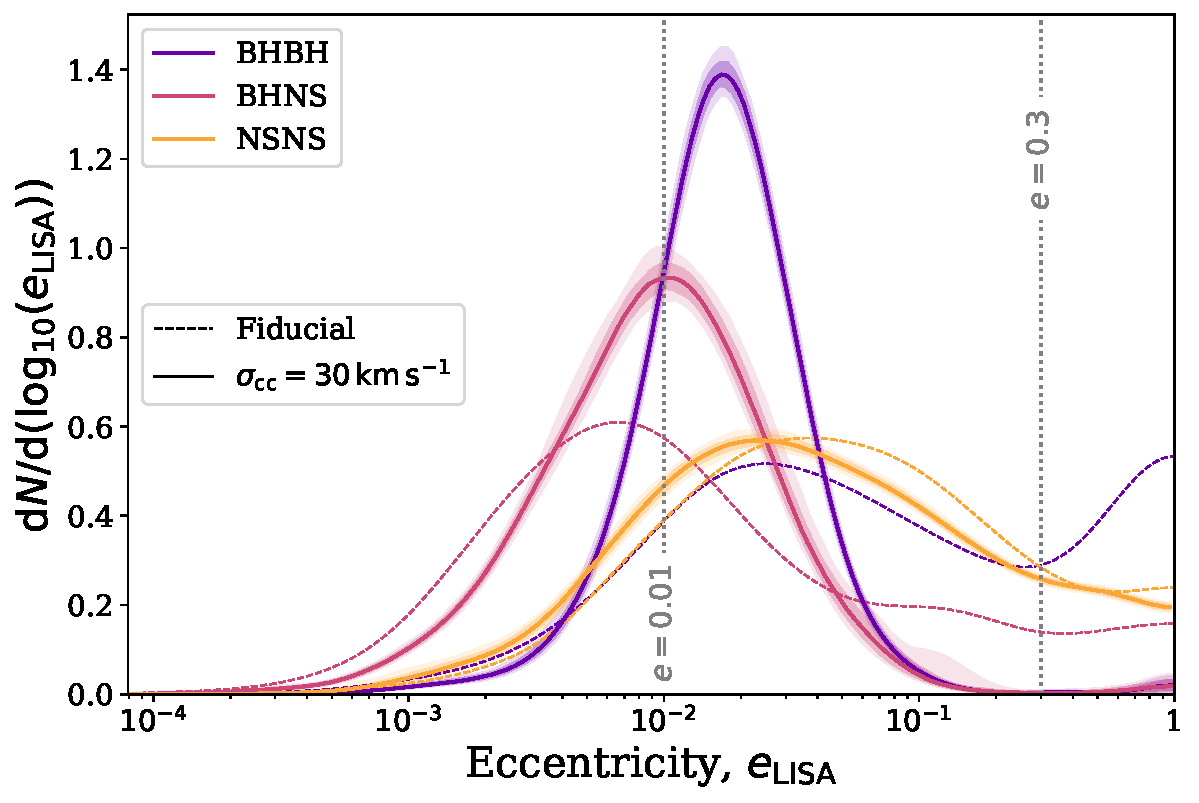
\includegraphics[width=\columnwidth]{ecc_low_kick_variation.pdf}
    \caption{As lower left panel of Fig.~\ref{fig:fiducial_pdf_distributions}, but for model \modSigLower{}. For comparison, we show the mean distribution for the fiducial model as dashed lines.}
    \label{fig:ecc_low_kick_variation}
\end{figure}

% \begin{table}[htb]
%     \centering
%     \begin{tabular}{l|cccc}
%         \hline
%         \multirow{2}{*}{Component} & At Formation & \multicolumn{3}{c}{LISA detectable (4 year)} \\ \cline{2-5}
%         & All & BHBH & BHNS & NSNS \\
%         \hline
%         Low-$\alpha$ disc & 42.5\% & 88.6\% & 81.8\% & 84.9\%\\
%         High-$\alpha$ disc & 42.5\% & 5.2\% & 8.1\% & 12.0\%\\
%         Bulge & 15.0\% & 6.2\% & 10.1\% & 3.1\%\\
%     \end{tabular}
%     \caption{Percentage of systems in each Galactic component.}
% \end{table}